% Options for packages loaded elsewhere
\PassOptionsToPackage{unicode}{hyperref}
\PassOptionsToPackage{hyphens}{url}
\PassOptionsToPackage{dvipsnames,svgnames,x11names}{xcolor}
\documentclass[
  11pt,
]{article}
\usepackage{xcolor}
\usepackage[margin=2.4cm]{geometry}
\usepackage{amsmath,amssymb}
\setcounter{secnumdepth}{-\maxdimen} % remove section numbering
\usepackage{iftex}
\ifPDFTeX
  \usepackage[T1]{fontenc}
  \usepackage[utf8]{inputenc}
  \usepackage{textcomp} % provide euro and other symbols
\else % if luatex or xetex
  \usepackage{unicode-math} % this also loads fontspec
  \defaultfontfeatures{Scale=MatchLowercase}
  \defaultfontfeatures[\rmfamily]{Ligatures=TeX,Scale=1}
\fi
\usepackage{lmodern}
\ifPDFTeX\else
  % xetex/luatex font selection
\fi
% Use upquote if available, for straight quotes in verbatim environments
\IfFileExists{upquote.sty}{\usepackage{upquote}}{}
\IfFileExists{microtype.sty}{% use microtype if available
  \usepackage[]{microtype}
  \UseMicrotypeSet[protrusion]{basicmath} % disable protrusion for tt fonts
}{}
\usepackage{setspace}
\makeatletter
\@ifundefined{KOMAClassName}{% if non-KOMA class
  \IfFileExists{parskip.sty}{%
    \usepackage{parskip}
  }{% else
    \setlength{\parindent}{0pt}
    \setlength{\parskip}{6pt plus 2pt minus 1pt}}
}{% if KOMA class
  \KOMAoptions{parskip=half}}
\makeatother
\setlength{\emergencystretch}{3em} % prevent overfull lines
\providecommand{\tightlist}{%
  \setlength{\itemsep}{0pt}\setlength{\parskip}{0pt}}
% v3 header: single column, tight reference list, clickable links.
% Loaded via pandoc -H. Fixes for the six issues Havid found in the v2 PDF are
% mostly in the markdown generator; this file only carries LaTeX-side settings.
\usepackage{graphicx}
\usepackage{float}
\usepackage{caption}

% Notation typesetting. Havid asked for consistency of format (2026-09-08),
% so units and species are expressed with the packages the field uses rather
% than a hand-rolled $^2$ regex table.
%
% VERIFIED before adoption: both compile under tectonic, which auto-downloads
% mhchem.sty and chemgreek.sty from its bundle -- no manual TeX Live install.
% Verified at PDF span level too: \qty{1.3e-3}{\centi\meter\squared\per\volt
% \per\second} raises every exponent AND every minus, and \ce{[PbI4]^2-} puts
% the subscript 4 BELOW the baseline with the charge ABOVE it in one token.
% A regex table cannot script one token in two directions.
%
% mhchem version=4 pinned: version 3 changed the charge syntax, so an
% unpinned load would silently alter every ion in the paper.
\usepackage{siunitx}
\usepackage[version=4]{mhchem}

% Journal-style units: upright glyphs, thin space between value and unit,
% and a real minus in exponents. detect-weight keeps units upright inside a
% bold heading instead of inheriting the surrounding bold.
\sisetup{
  detect-all,
  detect-weight        = true,
  range-units          = single,
  % reciprocal, NOT symbol. With per-mode=symbol the electron mobility
  % rendered as "cm2/(V s)", which is typographically correct but is not the
  % convention this literature uses; every perovskite paper writes
  % "cm2 V-1 s-1" with reciprocal powers. Verified at span level: reciprocal
  % raises both the 2 and each minus sign.
  per-mode             = reciprocal,
  exponent-product     = \times,
  output-decimal-marker = {.},
  group-digits         = none
}

% Figure captions: LaTeX owns the "Figure N." label. The v2 PDF rendered
% "Figure 4: Figure 4." because the caption text ALSO began with "Figure 4.",
% written into the markdown by the generator. v3 passes a bare caption and lets
% LaTeX number it, so the label appears exactly once.
\captionsetup[figure]{labelfont=bf, labelsep=period, font=small,
                      justification=justified, singlelinecheck=false,
                      skip=6pt}

% Tighten the numbered reference list produced by pandoc's default
% CSLReferences environment.
\usepackage{etoolbox}
\AtBeginEnvironment{CSLReferences}{%
  \small
  \setlength{\parskip}{0pt}%
  \setlength{\itemsep}{0pt}%
  \setlength{\topsep}{2pt}%
}

% No section numbering from LaTeX: the generator already writes "1. Introduction",
% "2. The Certified Frontier ...", so LaTeX numbering would double it.
\setcounter{secnumdepth}{0}
\usepackage{bookmark}
\IfFileExists{xurl.sty}{\usepackage{xurl}}{} % add URL line breaks if available
\urlstyle{same}
% fallback for those not using the hyperref driver hyperxmp:
\makeatletter
\@ifundefined{xmpquote}{\newcommand{\xmpquote}[1]{#1}}{}
\makeatother
\hypersetup{
  colorlinks=true,
  linkcolor={[HTML]{1A4E8A}},
  filecolor={Maroon},
  citecolor={Blue},
  urlcolor={[HTML]{1A4E8A}},
  pdfcreator={LaTeX via pandoc}}

\author{}
\date{}

\begin{document}

\setstretch{1.05}
\begin{center}
{\LARGE\bfseries Perovskite Photovoltaics in June 2026: Defect passivation, composition and phase control\par}
\vspace{1.1em}
{\large Havid Aqoma\textsuperscript{1,2,3,4,*}\par}
\vspace{0.7em}
\begin{minipage}{\textwidth}\centering\small
\textsuperscript{1}School of Energy and Chemical Engineering, Xiamen University Malaysia, Selangor Darul Ehsan 43900, Malaysia\\[0.25em]
\textsuperscript{2}Kelip-kelip! Center of Excellence for Light Enabling Technologies, School of Energy and Chemical Engineering, Xiamen University Malaysia, Selangor Darul Ehsan 43900, Malaysia\\[0.25em]
\textsuperscript{3}Centre of Excellence for Green and Advanced Technologies in Efficient Separations (GATES), School of Energy and Chemical Engineering, Xiamen University Malaysia, Selangor Darul Ehsan 43900, Malaysia\\[0.25em]
\textsuperscript{4}Gulei Innovation Institute, Xiamen University, Zhangzhou 363200, China\\[0.55em]
*Corresponding author. Email: havidaqoma.khoiruddin@xmu.edu.my\\[2.0em]
September 9, 2026
\end{minipage}
\end{center}
\vspace{0.8em}

\subsection{Abstract}\label{abstract}

An evaluation of 623 publications indexed during this monthly cycle,
with 167 examined in critical detail, reveals that perovskite
photovoltaic research remains divided between unverified laboratory
claims and corroborated physical mechanisms. Independent certification
remains scarce, as only 14 studies provide accredited performance data.
The verified efficiency ceiling reaches 33.6\% in monolithic tandem
architectures through dense self-assembled monolayer (SAM) contacts that
suppress buried-interface halide migration, whereas single-junction
devices attain 27.28\% through multidentate Lewis-base chelation of
undercoordinated lead cations. A pronounced area penalty emerges upon
device scaling: although uncertified small-area coupons assert higher
values, certified power conversion efficiency (PCE) falls to 26.8\% at
an aperture area of \qty{655.2}{\centi\meter}\(^2\) because localized
phase impurities, non-uniform film crystallization, and series
resistance penalize large-area charge collection. Operational stability
reporting exhibits severe evidentiary deficits, as only 6 investigations
document operational lifetime, with the longest sustained test achieving
\qty{3600}{\hour}, while only 5 adhere to standardized International
Summit on Organic Photovoltaic Stability (ISOS) protocols. This
reporting deficit extends across the literature: although 48.1\% of
abstracts state an efficiency, only 5.9\% report independent
certification, leaving most performance claims unshielded from
sweep-rate hysteresis, spectral mismatch, and transient capacitive
artifacts. Mechanistically, corroborated evidence converges on
multidentate coordination and stereochemical configuration to elevate
halide vacancy formation energies, distinguishing genuine deep trap
remediation from transient field-effect screening. In contrast, claims
of thermodynamic phase stabilization remain thin, as chemical additives
primarily introduce kinetic barriers or alter coherent interfacial
strain to delay conversion from the photoactive cubic phase to the
non-photoactive hexagonal phase. At selective contacts, hole extraction
depends on molecular ordering, catalytic chemisorption, and chemical
buffering against interfacial deprotonation rather than macroscopic
work-function tuning, which conceals severe nanoscale trap disorder.
Under operational electrical stress, non-recoverable decay stems from
coupled interfacial degradation, including electrode corrosion and
fullerene photo-oligomerization, demonstrating that unstandardized
steady-state characterization routinely conflates reversible ionic
polarization with permanent defect remediation.

\textbf{Keywords:} perovskite photovoltaics; buried interface; defect
passivation; wide-bandgap perovskite; tandem solar cells; operational
stability

\subsection{1. Introduction}\label{introduction}

Standard steady-state characterization cannot distinguish reversible
ionic redistribution from irreversible chemical decomposition, leaving
ambiguous whether reported passivation strategies eliminate
recombination centres or merely establish transient screening fields.
Resolving this ambiguity defines the central challenge in perovskite
photovoltaics, where the research frontier has departed from raw power
conversion efficiency (PCE) recorded on small-area coupons. Progress now
requires reproducible independent verification, structural uniformity
over scalable device areas, and operating lifetime that resists coupled
thermal, environmental, and electrical stress.

A total of 623 indexed works met the scope gate in June 2026 and 167
were read closely. Across this evidence base, this review distinguishes
what the month's literature verified through corroborated physical
measurement from what it asserted through uncalibrated fits, isolated
champion cells, or non-standard aging protocols.

Five mechanistic threads track the findings that withstand that
measurement uncertainty: non-radiative recombination and defect control,
crystallisation pathways and phase stability, interfacial energetics and
contact design, operational lifetime and failure pathways, and subcell
design and tandem interconnection. Tracing these processes clarifies
where microscopic defect passivation translates into authentic device
endurance, and where nominal performance gains remain artifacts of
measurement conditions.

\subsection{2. The Certified Frontier in June
2026}\label{the-certified-frontier-in-june-2026}

Unstandardized laboratory current-voltage measurements cannot
distinguish interfacial defect passivation from transient capacitive
currents, sweep-rate hysteresis, spectral mismatch, or aperture
misalignment. Only 14 of 167 closely read papers reported an
independently certified efficiency, leaving the majority of performance
claims unshielded from these experimental ambiguities. What survives
standardization establishes the verified photovoltaic ceiling.
Two-terminal (2T) tandems set the highest certified power conversion
efficiency (PCE) at 33.6\% and 32.95\%, with a lower certified baseline
at 28.79\%
{[}\href{https://doi.org/10.1126/science.aef5355}{1},\href{https://doi.org/10.1038/s41467-026-73276-w}{2},\href{https://doi.org/10.1002/anie.4918900}{3}{]}.
Unclassified cell architectures reach certified efficiencies of 27.28\%
and 26.84\%
{[}\href{https://doi.org/10.1126/sciadv.aef6596}{4},\href{https://doi.org/10.1038/s41467-026-74107-8}{5}{]},
while certified inverted (p-i-n) devices cap at 26.8\% and 26.44\%
{[}\href{https://doi.org/10.1002/adma.73855}{6},\href{https://doi.org/10.1021/acsenergylett.6c01257}{7}{]}.

For scalable modules, the certified ceiling drops to 26.61\%
{[}\href{https://doi.org/10.1002/aenm.71159}{8}{]}. Self-reported values
at large aperture areas run substantially ahead of this verified module
boundary, reaching 27.12\% on \qty{655.2}{\centi\meter\squared}
{[}\href{https://doi.org/10.1002/adma.73855}{6}{]}, 26.88\% on
\qty{29.7}{\centi\meter\squared}
{[}\href{https://doi.org/10.1038/s41467-026-74288-2}{9}{]}, 26.76\% on
\qty{12}{\centi\meter\squared}
{[}\href{https://doi.org/10.1002/adfm.76756}{10}{]}, 26.52\% on
\qty{50}{\centi\meter\squared}
{[}\href{https://doi.org/10.1002/anie.2974414}{11}{]}, and 26.13\% on
\qty{57.6}{\centi\meter\squared}
{[}\href{https://doi.org/10.1038/s41467-026-73276-w}{2}{]}. A champion
efficiency recorded on a tiny laboratory cell and an independently
certified efficiency measured at module area provide fundamentally
distinct physical evidence. The miniature laboratory cell interrogates
local non-radiative recombination suppression under negligible series
resistance and idealized collection geometries. By contrast, a certified
module reflects distributed transport physics, penalizing performance
through interconnect dead areas, sheet resistance across transparent
conductors, and film thickness gradients over large spans. Treating
micro-scale champion metrics as indicators of module feasibility
conflates intrinsic material quality with macroscopic charge-transport
management.

\begin{figure}[htbp]
\centering
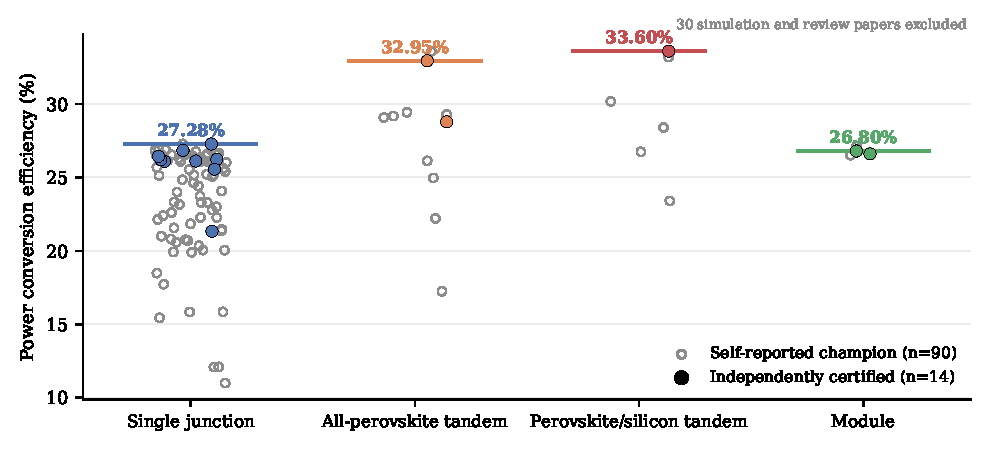
\includegraphics[width=0.95\textwidth]{fig/F1_certified_frontier.pdf}
\caption{The certified frontier in June 2026. Filled markers are independently certified efficiencies, open markers are self-reported champion values, grouped by device family. Horizontal bars mark the highest certified value in each family.}
\end{figure}

\subsection{3. Non-Radiative Recombination and Defect
Control}\label{non-radiative-recombination-and-defect-control}

Standard optoelectronic characterization cannot definitively separate
true chemical passivation of deep sub-gap trap states from electrostatic
band-bending, interfacial dipole reorientation, or suppressed mobile ion
accumulation that dynamically alters interface recombination. Most
reported open-circuit voltage (\(V_{\mathrm{oc}}\)) and
photoluminescence improvements conflate these effects. Evidence of
genuine chemical trap remediation survives where multidentate Lewis-base
chelators target undercoordinated lead (\(\mathrm{Pb}^{2+}\)) cations
and halide vacancies. Bidentate coordination directly elevates defect
formation energies and prevents ligand detachment: dabrafenib (DRFN)
binds multiple \(\mathrm{Pb}^{2+}\) centers through its sulfonyl group
and heterocyclic nitrogen to yield uncertified power conversion
efficiencies (power conversion efficiency (PCE)) of 25.28\% in n-i-p and
26.62\% in p-i-n cells
{[}\href{https://doi.org/10.1002/adfm.76623}{12}{]}, while dithiol
chelation (DPS) forms stable five-membered rings with
\(\mathrm{Pb}^{2+}\) to achieve 22.28\% PCE
{[}\href{https://doi.org/10.1002/adma.73833}{13}{]}. Enantiomeric
anchoring reveals that steric configuration dictates coordination
strength: chiral R-Pye raises the iodine vacancy formation energy from
2.46 to \qty{4.56}{\electronvolt} with a \qty{9.45}{\electronvolt}
binding energy compared to \qty{7.33}{\electronvolt} for S-Pye,
delivering 26.13\% PCE
{[}\href{https://doi.org/10.1002/aenm.71222}{14}{]}. Similarly,
functionalized aromatics like 2-amino-4,6-dichlorotriazine relieve
\(\mathrm{PbI}_6\) octahedral distortion while coordinating
\(\mathrm{Pb}^{2+}\) and halide vacancies (26.58\% PCE)
{[}\href{https://doi.org/10.1021/acsmaterialslett.5c01678}{15}{]},
paralleled by triazine anchoring that suppresses
\(\mathrm{Pb}\)-\(\mathrm{I}\) antisites
{[}\href{https://doi.org/10.1002/adfm.76218}{16}{]}, amino-pyridine
derivatives (ACA) strengthening \(\mathrm{Pb}^{2+}\) coordination via
electron donation while hydrogen-bonding lattice iodide (15.84\% PCE)
{[}\href{https://doi.org/10.1021/acs.jpclett.6c01600}{17}{]}, and
dual-site binding through carbonyl, phenolic, or cyano groups
{[}\href{https://doi.org/10.1021/acsami.6c04650}{18},\href{https://doi.org/10.1002/smll.74320}{19},\href{https://doi.org/10.1021/acs.jpclett.6c01458}{20}{]}.

This mechanistic picture is obscured when molecular treatments
simultaneously alter bulk crystal growth, leaving unclear whether
non-radiative recombination decreases from localized defect passivation
or reduced grain boundary area. The dual-functional ionic liquid PIT
decouples these actions: its anion coordinates \(\mathrm{Pb}^{2+}\) and
organic cations, whereas its cation segregates to the upper surface to
retard crystallization and enlarge grains, achieving 25.94\% PCE
{[}\href{https://doi.org/10.1002/smll.74328}{21}{]}. Co-passivation with
potassium diformate and potassium phosphate similarly halves trap
density while expanding grain size from 780 to \qty{1370}{\nano\meter}
(24.42\% PCE) {[}\href{https://doi.org/10.1021/acsami.6c06698}{22}{]}.
At buried contacts, separating chemical passivation from nucleation
control remains equally challenging. Adding \(\mathrm{CsPbBr}_3\)
nanocrystal seeds passivates the buried interface while steering
crystallization, yielding 24.63\% PCE against 22.89\% for unseeded
controls {[}\href{https://doi.org/10.1002/smll.74279}{23}{]}.
Interfacial polymeric interlayers like ultraviolet (UV)-crosslinked RM82
diacrylates passivate buried tin oxide (\(\mathrm{SnO}_2\)) interfaces
while promoting crystal growth, though reported stability relies on
passive ambient storage rather than operational stress
{[}\href{https://doi.org/10.1021/acsaem.6c00330}{24}{]}. CTW-g-PANI
coordinates undercoordinated tin sites to heal \(\mathrm{SnO}_x\) oxygen
vacancies and passivate surface perovskite states (17.73\% PCE)
{[}\href{https://doi.org/10.1021/acsami.6c05326}{25}{]}. In tin-lead
perovskites, differential chelation resolves mismatched crystallization
kinetics: 1,10-phenanthroline binds \(\mathrm{Sn}^{2+}\) preferentially
over \(\mathrm{Pb}^{2+}\), synchronizing film growth to achieve an
uncertified 23.63\% PCE, 81.27\% fill factor (FF), and
\qty{0.887}{\volt} \(V_{\mathrm{oc}}\)
{[}\href{https://doi.org/10.1002/eem2.70453}{26}{]}.

Static defect metrics also cannot distinguish permanent electronic trap
deactivation from temporary trap filling or the suppression of
field-driven ion migration. Although illumination-assisted trap filling
achieves long electron lifetimes up to 547 ± 9 µs in polycrystalline
films {[}\href{https://doi.org/10.1002/adfm.76273}{27}{]}, unpassivated
mobile ions migrate under operational bias to generate new recombination
centers. Defect suppression only survives long-term operation when ion
migration pathways are physically sealed. 2PyS coordination suppresses
undercoordinated \(\mathrm{Pb}^{2+}\) and halide vacancies, limiting ion
drift and preserving over 91\% efficiency after \qty{2000}{\hour} in
wide-bandgap (WBG) cells
{[}\href{https://doi.org/10.1088/2752-5724/ae7817}{28}{]}, consistent
with molecular confinement domains restricting formamidinium motion to
arrest halide segregation (24.21\% and 21.20\% PCE for 1.68 and
\qty{1.78}{\electronvolt} bandgaps)
{[}\href{https://doi.org/10.1002/adma.73713}{29}{]}. Time-of-flight
secondary ion mass spectrometry (ToF-SIMS) confirms that multidentate
ATZCl forms a Ruddlesden-Popper (RP)-like surface phase that blocks
iodide migration across the hole transport layer (hole-transport layer
(HTL)) (25.22\% PCE)
{[}\href{https://doi.org/10.1021/acs.nanolett.6c00804}{30}{]}. Replacing
small molecules with in situ polymerized vinylphosphonic acid provides a
rare certified 26.24\% PCE (26.54\% uncertified champion) with over 90\%
retention after \qty{1600}{\hour} of continuous maximum power point
tracking (MPPT) {[}\href{https://doi.org/10.1002/adma.202522825}{31}{]},
demonstrating that covalent network immobilization prevents
field-induced passivator detachment and settles the ambiguity between
chemical trap deactivation and dynamic ion blocking.

\begin{figure}[htbp]
\centering
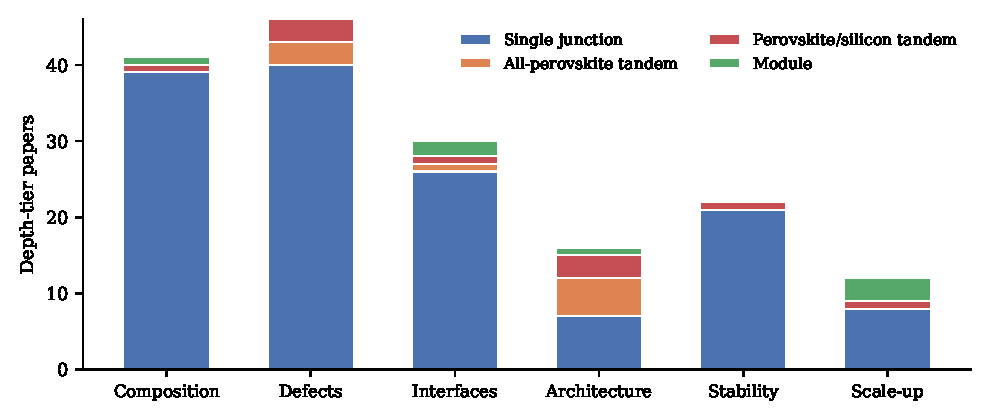
\includegraphics[width=0.95\textwidth]{fig/F3_effort_map.pdf}
\caption{Where the month's mechanistic effort was directed. Depth-tier papers by mechanism axis, stacked by device family.}
\end{figure}

\subsection{4. Crystallisation Pathways and Phase
Stability}\label{crystallisation-pathways-and-phase-stability}

Bulk structural probes cannot distinguish whether additives genuinely
alter the thermodynamic free-energy landscape of perovskite phases or
merely impose kinetic barriers that freeze metastable states
{[}\href{https://doi.org/10.22541/authorea.15004927/v1}{32}{]}.
Spatially averaged X-ray diffraction (XRD) routinely masks localized
phase impurities, while thermal calibration offsets skew the
determination of true phase-transition and decomposition onsets in
halide powders
{[}\href{https://doi.org/10.22541/authorea.15004927/v1}{32},\href{https://doi.org/10.48550/arxiv.2606.27592}{33}{]}.
What survives this diagnostic ambiguity is that local interfacial
lattice matching and coherent strain govern polymorphic stability. In
formamidinium lead triiodide (\ce{FAPbI3}), the spontaneous conversion
from the photoactive black cubic perovskite (α-phase) to the
non-photoactive yellow hexagonal (δ-phase) at room temperature nucleates
at coherent interfaces between α-phase (011) and δ-phase (110) planes
under tensile strain
{[}\href{https://doi.org/10.1038/s41467-026-73739-0}{34},\href{https://doi.org/10.1002/solr.70396}{35}{]}.
Introducing two-dimensional (2D) perovskitoid interlayers disrupts this
preferred δ-phase orientation, yielding an uncertified 25.61\% champion
power conversion efficiency (PCE)
{[}\href{https://doi.org/10.1038/s41467-026-73739-0}{34}{]}. Interfacial
strain regulation is equally achieved by constructing one-dimensional
(1D) THAPbI3 heterojunctions using tetrahexylammonium iodide (THAI),
which anchors formamidinium (FA+) cations through hydrogen bonding to
suppress outward cation diffusion and strain gradients, achieving an
uncertified 25.06\% PCE on unstated cell dimensions
{[}\href{https://doi.org/10.1021/acsaem.6c01363}{36}{]}. Transient
intermediate phases also dictate phase-pure crystallization pathways.
Volatile thiocyanate (SCN-) anions transiently coordinate with lead
(\ce{Pb^2+}) precursors to restructure crystallization kinetics; while
ammonium (\ce{NH4}+) cations volatilize during thermal annealing to
drive bulk grain enlargement, residual phenylethylammonium (PEA+)
cations segregate to grain boundaries to provide surface passivation,
achieving 23.3\% PCE
{[}\href{https://doi.org/10.1021/acsaem.6c01329}{37}{]}. In
all-inorganic cesium lead triiodide (\ce{CsPbI3}), formamidinium acetate
(FAAC) reduces the formation energy of the Cs4PbI6 intermediate phase,
facilitating complete dimethylammonium (DMA+) to cesium (\ce{Cs+})
cation exchange and accelerating dimethylammonium iodide (DMAI) removal
to yield 21.84\% PCE
{[}\href{https://doi.org/10.1021/acs.jpclett.6c01395}{38}{]}.

In wide-bandgap mixed-halide absorbers, measurements similarly struggle
to distinguish growth-induced compositional heterogeneity from
operational light-induced phase segregation
{[}\href{https://doi.org/10.22541/authorea.15004927/v1}{32},\href{https://doi.org/10.1016/j.xcrp.2026.103346}{39}{]}.
Resolving this requires synchronizing disparate halide crystallization
kinetics. Eutectic urea phosphate, possessing stronger affinity for
bromine-based over iodine-based octahedra, equalizes reaction rates to
eliminate vertical and lateral phase segregation, yielding 22.27\% PCE
{[}\href{https://doi.org/10.1002/anie.2535666}{40}{]}. Epitaxial growth
on spinel oxide substrates uses lattice matching and magnesium-halide
interfacial bonds to induce compressive strain, which arrests halide
segregation without organic additives
{[}\href{https://doi.org/10.1021/jacs.6c04846}{41}{]}. For
multi-junction absorbers, substituting bromide with chloride in
Cs0.05(FA0.90MA0.10)0.95Pb(I0.95Br0.05)3 (incorporating methylammonium,
MA+) circumvents performance losses observed beyond
\qty{450}{\nano\meter} thickness, enabling crack-free vertical
crystallization up to \textasciitilde{}\qty{700}{\nano\meter} without
sacrificing fill factor (FF) or open-circuit voltage (Voc) to achieve
23.4\% PCE on a \qty{1}{\centi\meter\squared} aperture
{[}\href{https://doi.org/10.1002/solr.70410}{42}{]}.

Controlling orientation templates is critical for dimensional stability.
Templated crystallization using pre-synthesized large-area n = 1 2D
perovskite nanosheets drives three-dimensional (3D) film growth with
high crystallinity and preferred orientation, achieving 21.36\% PCE
(20.75\% stabilized power output) and a hysteresis coefficient below 1\%
{[}\href{https://doi.org/10.1002/smll.74076}{43}{]}. Propylammonium
iodide (PAI) added during two-step blade coating directs (111)-oriented
growth in inverted cells, delivering 20.05\% PCE and retaining 95\% of
initial efficiency over \qty{1680}{\hour} of maximum power point
tracking (MPPT) {[}\href{https://doi.org/10.1002/solr.70385}{44}{]}.
Conversely, solvent-additive approaches such as rubidium chloride (RbCl)
in 2-methoxyethanol and dimethylacetamide (DMAc) claim methylammonium
lead triiodide (\ce{MAPbI3}) phase regulation, yet stability
verification is limited to \qty{300}{\second} of steady-state output at
18.48\% PCE {[}\href{https://doi.org/10.1002/solr.70363}{45}{]}. In
quasi-2D systems, functional group configuration in isomeric additives
dictates molecular stacking: cytosine exhibits stronger delocalized
interactions than iso-cytosine, facilitating favorable nucleation to
attain 22.4\% PCE with a T80 lifetime (time to 80\% initial efficiency)
of \qty{3600}{\hour}
{[}\href{https://doi.org/10.1021/acs.jpclett.6c01531}{46}{]}.
Intermolecular pi-pi interactions in 3,3'-methylenediphenyldiammonium
cations stabilize a non-Dion-Jacobson (non-DJ) 2D perovskite, yielding
26.52\% module PCE on \qty{50}{\centi\meter\squared}
{[}\href{https://doi.org/10.1002/anie.2974414}{11}{]}. For tin-based
perovskites, density functional theory (DFT) guided screening of solvent
vapor fuming identifies tetramethylurea (TMU), which slows coordination
kinetics to enable carrier extraction in 0.67 μs and a 75.14 μs
recombination lifetime, reaching 10.45\% PCE
{[}\href{https://doi.org/10.1021/acsenergylett.6c01505}{47}{]}.

\subsection{5. Interfacial Energetics and Contact
Design}\label{interfacial-energetics-and-contact-design}

Macroscopic junction characterizations fail to distinguish whether
contact modifications enhance carrier collection through electrostatic
band alignment or through the physical elimination of local pinholes,
solvent washouts, and interfacial deprotonation. Transient photovoltage
and photocurrent mapping reveals that inhomogeneous hole transport layer
(hole-transport layer (HTL)) junctions generate trapped-hole densities
up to \qty{1.6e17}{\per\centi\meter\cubed}
{[}\href{https://doi.org/10.1021/acsaem.6c00612}{48}{]}, confirming that
macroscopic work function shifts routinely conceal severe nanoscale
contact disorder. Under operational stress, unimolecular self-assembled
monolayer (SAM) contacts undergo severe degradation driven by
thermomechanical mismatch with the perovskite absorber
{[}\href{https://doi.org/10.1038/s44172-026-00695-4}{49}{]}. What
survives this diagnostic ambiguity is direct evidence that contact
durability depends on molecular ordering, multi-site anchoring, and
chemical buffering against proton transfer rather than energetic tuning
alone.

Because casting perovskite precursor solutions washes away unanchored
molecules, contact integrity requires accelerated chemisorption or
continuous replenishing. Catalytic deposition using
4-dimethylaminopyridine (DMAP) accelerates phosphonic acid binding to
indium tin oxide (ITO) via phosphorylpyridinium intermediates, achieving
a certified power conversion efficiency (PCE) of 26.44\% (champion
26.93\%) {[}\href{https://doi.org/10.1021/acsenergylett.6c01257}{7}{]},
while directly doping SAM molecules into precursor solutions or
inserting alumina nanoparticles counters solvent erosion and seals
pinholes
{[}\href{https://doi.org/10.1021/acsami.6c02373}{50},\href{https://doi.org/10.1002/smll.74200}{51}{]}.
At the substrate interface, uniform coverage requires suppressing
molecular agglomeration; bisphosphonic anchors, seed layers, and
rigidified conjugated backbones enforce packing uniformity and favorable
dipole alignment without excessive islanding
{[}\href{https://doi.org/10.1002/adfm.76418}{52},\href{https://doi.org/10.1002/adma.73567}{53},\href{https://doi.org/10.1002/adfm.76243}{54},\href{https://doi.org/10.1002/smll.74278}{55}{]}.
Specifically, rigid phenyl linkers elevate champion PCE to 23.30\%
compared to 22.38\% for flexible alkyl analogues
{[}\href{https://doi.org/10.1002/adfm.76243}{54}{]}, and nonplanar
butterfly geometries maintain 97.5\% efficiency after \qty{1000}{\hour}
under International Summit on Organic Photovoltaic Stability (ISOS)
ISOS-L-1 testing {[}\href{https://doi.org/10.1002/smll.74278}{55}{]}. To
resist interfacial shearing, multidentate and polymeric architectures
buffer stress: a multidentate phosphonic acid network boosts fracture
toughness nearly eightfold to 9.11 MPa (certified 26.61\% PCE, though on
an unscaled \qty{0.06734}{\centi\meter\squared} area)
{[}\href{https://doi.org/10.1002/aenm.71159}{8}{]}, whereas polymeric
Poly-3Ph-4PACz delivers 22.22\% PCE on \qty{57.6}{\centi\meter\squared}
flexible modules
{[}\href{https://doi.org/10.1038/s41467-026-73276-w}{2}{]}.

At electron transport layer (electron-transport layer (ETL)) contacts,
performance gains are frequently misattributed to work function
realignment when chemical degradation dominates. Basic hydroxyls on tin
oxide (\ce{SnO2}) promote formamidinium (FA+) deprotonation, a failure
mode arrested by phosphate buffering or hydrogen-bonding additives at
buried junctions
{[}\href{https://doi.org/10.1002/aenm.71170}{56},\href{https://doi.org/10.1021/acssuschemeng.6c04546}{57}{]}.
Concurrently, bilateral functional molecules mitigate interface trap
states by coordinating uncoordinated lead ions while covalently
anchoring oxide hydroxyls
{[}\href{https://doi.org/10.1002/smll.202510785}{58},\href{https://doi.org/10.1002/advs.76010}{59}{]}.
Uncertified champion devices with L-isoleucine modification reach
26.15\% PCE versus 23.54\% for controls
{[}\href{https://doi.org/10.1002/smll.202510785}{58}{]}, while
sulfonated bathocuproine derivatives suppress recombination through
combined sodium-ion and pyridinic coordination to reach 26.02\% PCE
{[}\href{https://doi.org/10.1002/advs.76010}{59}{]}. Decoupling bulk
crystallization from interfacial reconstruction via triple-alkali
interlayers provides an open-circuit voltage (Voc) of \qty{1.184}{\volt}
and 83.81\% fill factor (champion 26.13\% PCE)
{[}\href{https://doi.org/10.1002/adma.73535}{60}{]}, demonstrating that
chemical restructuring of the contact outweighs electrostatic band
alignment.

\subsection{6. Operational Lifetime and Failure
Pathways}\label{operational-lifetime-and-failure-pathways}

Standard operational metrics fail to distinguish reversible ionic
polarization from catastrophic degradation under electrical stress,
where cells with poly(triarylamine) (PTAA) suffer irreversible breakdown
under reverse current near maximum power point (MPP) while
carbazole-based monolayers show recoverable decay
{[}\href{https://doi.org/10.1021/acsenergylett.6c00904}{61}{]}. This
diagnostic ambiguity is exacerbated by unstandardized testing: only 6 of
167 closely read studies reported a time to 80\% initial efficiency
(T80), and only 5 specified International Summit on Organic Photovoltaic
Stability (ISOS) protocols
{[}\href{https://doi.org/10.1126/sciadv.aef6596}{4},\href{https://doi.org/10.1016/j.cej.2026.177834}{62},\href{https://doi.org/10.1021/acsaem.6c00778}{63}{]}.
Unmonitored aging conceals whether decay originates from intrinsic soft
lattice dynamics
{[}\href{https://doi.org/10.1021/acsenergylett.6c01303}{64}{]} or
external weathering, where outdoor testing of a triple-junction cell
showed efficiency losses to 80\% at 4 months and 50\% at 6 months
{[}\href{https://doi.org/10.1002/solr.70390}{65}{]}. Accelerated stress
reproducing 20 months of outdoor operation demonstrates that varying
light intensity and bias drives three coexisting, spatially non-uniform
degradation modes: copper corrosion, edge patterns, and phase
segregation
{[}\href{https://doi.org/10.1016/j.joule.2026.102538}{66}{]}.

What survives this ambiguity is the mechanistic identification of
non-recoverable interfacial failure. At electron-transport interfaces,
phenyl-C61-butyric acid methyl ester (PCBM) undergoes photo-induced
{[}2+2{]} cycloaddition, causing dimerization and morphological
instability that steric additives suppress in uncertified 26.6\%
efficiency devices {[}\href{https://doi.org/10.1002/solr.70405}{67}{]}.
At hole-transport interfaces, chemical degradation dominates: unanchored
lithium ions migrate unless coordinated by sulfur centers, which
preserve approximately 90\% of initial efficiency across
\qty{800}{\hour} of MPP tracking (maximum power point tracking (MPPT))
under thermal and light stress, albeit on
\qty{0.04}{\centi\meter\squared} areas
{[}\href{https://doi.org/10.1002/adfm.76257}{68}{]}. Concurrently,
self-assembled monolayer (SAM) destabilization is prevented either by
transient two-dimensional (2D) capping layers that scale to 22.34\%
efficiency across \qty{615.7}{\centi\meter\squared} modules or by
hydroxylated MXene additives that strengthen SAM chemisorption on
\qty{0.0524}{\centi\meter\squared} cells
{[}\href{https://doi.org/10.1002/adma.73561}{69},\href{https://doi.org/10.1002/adma.73656}{70}{]}.

Beyond interfaces, degradation is governed by deep-level rather than
shallow defects: interstitial lead and formamidinium antisites dominate
non-radiative losses despite concentrations three orders of magnitude
lower than shallow states
{[}\href{https://doi.org/10.1002/adma.73679}{71}{]}. When exposed to
operational heat, bulky surface passivators induce localized lattice
expansion {[}\href{https://doi.org/10.1126/sciadv.aef6596}{4}{]},
whereas strain-regulating additives enable unencapsulated devices to
retain 80.5\% efficiency after \qty{1000}{\hour} at 85°C under ISOS-D-2I
and over 94.36\% after \qty{1500}{\hour} of MPPT under ISOS-L-1I
{[}\href{https://doi.org/10.1002/adfm.76756}{10}{]}.

\begin{figure}[htbp]
\centering
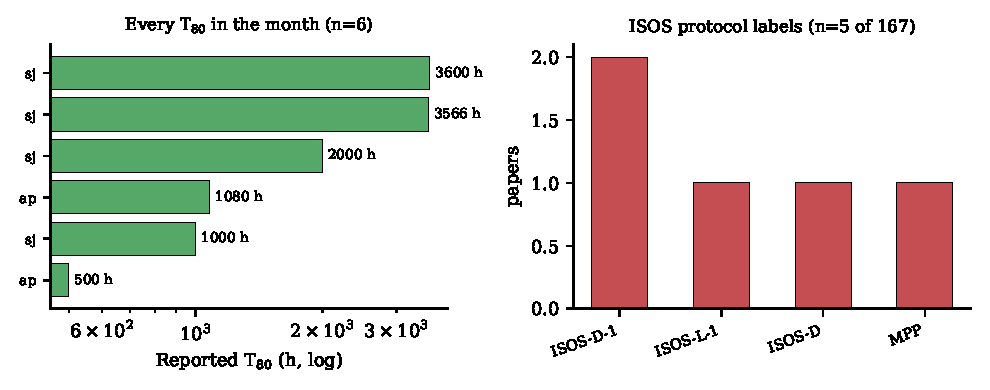
\includegraphics[width=0.95\textwidth]{fig/F4_stability_evidence.pdf}
\caption{The month's operational-stability evidence in full. Left, every reported time to 80\% of initial performance. Right, the stability protocol labels used.}
\end{figure}

\subsection{7. Subcell Design and Tandem
Interconnection}\label{subcell-design-and-tandem-interconnection}

Macroscopic current-voltage measurements cannot distinguish benign
structural disorder from performance-limiting defects: five sequentially
evaporated scaffolds yielded identical single-junction power conversion
efficiency (PCE) of about 19\% (supporting an uncertified 28.4\%
champion tandem PCE) despite marked disparities in conversion, halide
distribution, and morphology
{[}\href{https://doi.org/10.1021/acsami.6c07582}{72}{]}. Nor can
standard diagnostics separate electronic losses from mechanical fatigue,
as bending stress in flexible all-perovskite tandems (uncertified
champion PCE of 24.97\%) accelerates non-radiative recombination
detectable by grazing-incidence X-ray diffraction (GIXRD) well before
crack formation {[}\href{https://doi.org/10.1021/acsami.6c05001}{73}{]}.
What survives this ambiguity is that targeted chemical passivation and
redox regulation reliably mitigate recombination and ion migration
across buried contacts
{[}\href{https://doi.org/10.1126/science.aef5355}{1},\href{https://doi.org/10.1002/anie.4918900}{3},\href{https://doi.org/10.1038/s41467-026-74288-2}{9}{]}.
Anchoring dense self-assembled monolayer (SAM) coatings on reactive
plasma deposition (RPD)-grown tin oxide (SnOx) suppresses halide
migration in indium-free perovskite/silicon tandems, securing a
certified PCE of 33.6\% (uncertified champion 33.2\% on
\qty{1}{\centi\meter\squared}) and certified 31.0\% on a
\qty{207.9}{\centi\meter\squared} minimodule
{[}\href{https://doi.org/10.1126/science.aef5355}{1}{]}. At hole
contacts, neutralized alkali metal-based phosphonate salts (2PACz-M)
mixed with Me-4PACz delocalize interfacial charge across
\qty{29.7}{\centi\meter\squared} modules (uncertified champion 26.88\%
PCE) {[}\href{https://doi.org/10.1038/s41467-026-74288-2}{9}{]}, while
embedding allylthiourea (ATU) into
poly(3,4-ethylenedioxythiophene):poly(styrenesulfonate) (PEDOT:PSS)
enables dynamic iodine recycling, yielding a certified 28.79\% PCE
(uncertified champion 29.29\%)
{[}\href{https://doi.org/10.1002/anie.4918900}{3}{]}. In narrow-bandgap
subcells, Lewis coordination and seeding templates converge to govern
crystallite growth: Lewis hard-basicity amplification achieved an
uncertified 23.71\% single-junction PCE and an uncertified 29.44\%
champion tandem PCE with an uncertified time to 80\% initial efficiency
(T80) of \qty{1080}{\hour}
{[}\href{https://doi.org/10.1002/adma.73682}{74}{]}, while hybrid
\ce{CsPbBr3} quantum dot and metal-organic framework templates raise
fill factor (FF) above 81\% (uncertified 23.32\% single-junction PCE;
uncertified 29.18\% tandem PCE, uncertified T80 of \qty{500}{\hour})
{[}\href{https://doi.org/10.1002/anie.5595275}{75}{]}. For scale-up,
these chemical formulations endure atmospheric and mechanical stress:
blade coating with low-hygroscopic alcohol-alkane mixtures at 80\%
relative humidity achieves a certified 26.1\% PCE
{[}\href{https://doi.org/10.1038/s41467-026-72581-8}{76}{]}, while
dynamic-bond cross-linking monomers permit self-curing at 40°C for
\qty{30}{\minute} to deliver a certified 26.8\% PCE (uncertified
champion 27.12\%) on \qty{655.2}{\centi\meter\squared} flexible modules
{[}\href{https://doi.org/10.1002/adma.73855}{6}{]}.

\begin{figure}[htbp]
\centering
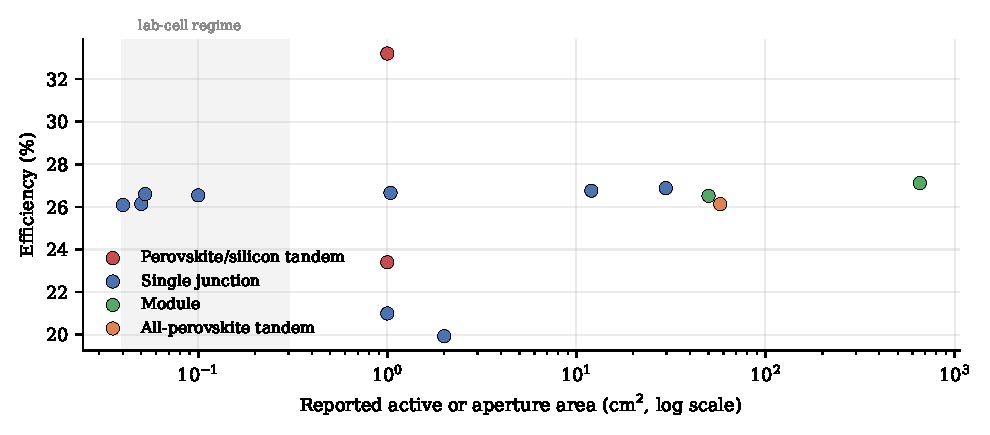
\includegraphics[width=0.95\textwidth]{fig/F2_area_penalty.pdf}
\caption{Efficiency against reported active or aperture area. The shaded band marks the sub-0.3 cm$^2$ laboratory-cell regime in which most champion values are measured.}
\end{figure}

\subsection{8. Research Gaps and
Outlook}\label{research-gaps-and-outlook}

Standard characterization cannot separate electronic defect remediation
from transient ionic polarization or kinetic phase trapping. Certified
power conversion efficiency (PCE) reached 33.6\% in two-terminal (2T)
tandems {[}\href{https://doi.org/10.1126/science.aef5355}{1}{]} and
26.8\% across a \qty{655.2}{\centi\meter\squared} aperture
{[}\href{https://doi.org/10.1002/adma.73855}{6}{]}, yet only 14 of 167
closely read papers reported certified values, leaving most performance
claims unresolved against measurement artifacts.

First, standard optoelectronic characterization fails to establish
whether Lewis-base chelators permanently remediate deep sub-gap traps or
merely induce transient field-effect screening
{[}\href{https://doi.org/10.1002/adfm.76623}{12}{]}. Differentiating
true chemical de-trapping from dynamic ionic screening requires
operando, bias-dependent drive-level capacitance profiling (DLCP) across
hole transport layer (hole-transport layer (HTL)) junctions, where
interfacial trapped-hole densities reach
\qty{1.6e17}{\per\centi\meter\cubed}
{[}\href{https://doi.org/10.1021/acsaem.6c00612}{48}{]}.

Second, bulk structural probes do not establish whether
strain-regulating additives shift the equilibrium free-energy landscape
or merely impose kinetic barriers that freeze metastable phases
{[}\href{https://doi.org/10.22541/authorea.15004927/v1}{32}{]}. Proving
whether interfacial coherent strain suppresses yellow non-perovskite
phase nucleation requires in situ high-pressure synchrotron X-ray
diffraction (XRD) paired with differential scanning calorimetry
calibrated against absolute transition enthalpies
{[}\href{https://doi.org/10.1038/s41467-026-73739-0}{34}{]}.

Third, unstandardized operational metrics fail to establish the boundary
separating reversible ionic polarization from catastrophic degradation
under electrical stress
{[}\href{https://doi.org/10.1021/acsenergylett.6c00904}{61}{]}. Only 6
papers reported a time to 80\% initial efficiency (T80) lifetime
(longest \qty{3600}{\hour}) and only 5 papers named an International
Summit on Organic Photovoltaic Stability (ISOS) protocol
{[}\href{https://doi.org/10.1126/sciadv.aef6596}{4},\href{https://doi.org/10.1016/j.joule.2026.102538}{66}{]}.
Closing this gap demands operando impedance spectroscopy tracking
equivalent-circuit transport parameters during cyclic ISOS reverse-bias
stress
{[}\href{https://doi.org/10.1126/sciadv.aef6596}{4},\href{https://doi.org/10.1021/acsenergylett.6c00904}{61}{]}.

Fourth, macroscopic current-voltage scans cannot establish which
morphological disparities in sequentially deposited scaffolds penalize
carrier collection
{[}\href{https://doi.org/10.1021/acsami.6c07582}{72}{]}. Although
scale-up was addressed by 24 of 623 works, identifying
performance-limiting defects over large areas requires spatially
resolved photoconductive atomic force microscopy correlated with local
photoluminescence quantum yields across device apertures up to
\qty{655.2}{\centi\meter\squared}
{[}\href{https://doi.org/10.1002/adma.73855}{6}{]}.

Next month's literature would be far more comparable if authors reported
certified steady-state power tracking on standardized aperture masks
alongside accredited T80 lifetimes under designated ISOS stress
protocols.

\subsection{Acknowledgements}\label{acknowledgements}

The authors would like to acknowledge the financial support from Xiamen
University Malaysia through the Xiamen University Malaysia Research Fund
(XMUMRF/2022-C10/IENG/0046), and from National Natural Science
Foundation of China (Ref. No.: 52503390).

\subsection{Declaration of Competing
Interest}\label{declaration-of-competing-interest}

The authors declare no conflict of interest.

\subsection{Data Availability
Statement}\label{data-availability-statement}

The corpus table for the month, the per-paper extraction records with
their verbatim source quotations, the statistics file underlying every
number in the text, and the gate report are provided as Supplementary
Information. Abstract text and full texts are not redistributed.

\subsection{AI Usage Declaration}\label{ai-usage-declaration}

This manuscript was prepared as part of our Research Project for making
a reliable Autonomous Researcher Agent. The agent executed the monthly
review pipeline without human intervention: it harvested the indexed
literature for the month through the OpenAlex, Semantic Scholar,
Crossref and arXiv interfaces, applied a deterministic topical filter,
ranked and selected the papers read closely, extracted every
quantitative claim into a structured record binding each number to a
verbatim quotation from that paper's own abstract, computed the
statistics and figures from those records, and drafted this text from
the resulting evidence briefs. Literature harvesting, selection,
statistics, figures and gate checking are deterministic scripts rather
than model output. Structured extraction used qwen3.8-flash through the
opencode interface; the prose was written by gemini-3.8-flash-high
through the agy interface; independent review used Opus 5 at high
reasoning effort. No figure is a model-generated image: every panel is
plotted directly from the extracted records. Every quantitative
statement in the main text resolves to the machine-generated statistics
file shipped as Supplementary Information, and every citation resolves
to a record carrying its source quotation. The author reviewed and
edited the content, verified the selection, and takes full
responsibility for the content of the published article.

\subsection{References}\label{references}

\begin{enumerate}
\def\labelenumi{\arabic{enumi}.}
\tightlist
\item
  Shi, W. et al.~Indium-free perovskite/silicon tandem solar cells with
  tin oxide recombination layer and electrodes. \emph{Science} (2026).
  \url{https://doi.org/10.1126/science.aef5355}
\item
  Tang, Q. et al.~Buried-interface homogenization by asymmetric
  polymeric self-assembled layers powers efficient, durable flexible
  perovskite photovoltaics. \emph{Nature Communications} (2026).
  \url{https://doi.org/10.1038/s41467-026-73276-w}
\item
  Zeng, M. et al.~Buried‐Interface Iodine Redox Regulation for Durable
  All‐Perovskite Tandem Photovoltaics. \emph{Angewandte Chemie
  International Edition} (2026).
  \url{https://doi.org/10.1002/anie.4918900}
\item
  Ren, Z. et al.~Reactive reconstruction and embedded passivation of
  heterointerfaces for intrinsically stable perovskite photovoltaics.
  \emph{Science Advances} (2026).
  \url{https://doi.org/10.1126/sciadv.aef6596}
\item
  Wen, Y. et al.~Indium-Based Octahedra Coordinating Pb--I Termini for
  Stable Perovskites. \emph{Nature Communications} (2026).
  \url{https://doi.org/10.1038/s41467-026-74107-8}
\item
  Huang, S. et al.~Molecularly Engineered Self‐Healing Scaffold With
  Customized Dynamic Bonds Enable Stable and Scalable Flexible
  Perovskite Solar Cells and Modules. \emph{Advanced Materials} (2026).
  \url{https://doi.org/10.1002/adma.73855}
\item
  Liu, Z. et al.~Kinetic Enhancement of Self-Assembled Molecular
  Deposition via Catalytic Additive for Inverted Perovskite Solar Cells.
  \emph{ACS Energy Letters} (2026).
  \url{https://doi.org/10.1021/acsenergylett.6c01257}
\item
  Hou, M. et al.~Mitigating Photothermal‐Induced Burn‐In in Perovskite
  Solar Cells via a Multidentate Phosphonic Acid Polymer Network.
  \emph{Advanced Energy Materials} (2026).
  \url{https://doi.org/10.1002/aenm.71159}
\item
  Yang, Y. et al.~Ionic self-assembled monolayers enable neutral
  interfaces and synergistic charge extraction in high-efficiency
  perovskite solar cells. \emph{Nature Communications} (2026).
  \url{https://doi.org/10.1038/s41467-026-74288-2}
\item
  Yang, Q. et al.~Regulating the Crystallization‐Defect‐Strain Improves
  the Stability and Scalability of FACs Perovskite Photovoltaics.
  \emph{Advanced Functional Materials} (2026).
  \url{https://doi.org/10.1002/adfm.76756}
\item
  Y, L. et al.~A Diammonium‐Based Non‐Dion‐Jacobson Phase 2D Perovskite
  With High Durability for Efficient and Stable 2D/3D Perovskite Solar
  Modules. \emph{Angewandte Chemie International Edition} (2026).
  \url{https://doi.org/10.1002/anie.2974414}
\item
  Dai, Y. et al.~Redox‐Driven Spatiotemporal Passivation for Efficient
  and Durable Perovskite Solar Cells. \emph{Advanced Functional
  Materials} (2026). \url{https://doi.org/10.1002/adfm.76623}
\item
  冯湘涵, et al.~Molecular Chelating‐Clamp Strategy Using Dithiol
  Antidotes Enables Efficient and Stable Inorganic Perovskite Solar
  Cells. \emph{Advanced Materials} (2026).
  \url{https://doi.org/10.1002/adma.73833}
\item
  Wang, R. et al.~Chiral Molecular Configuration‐Mediated
  Crystallization of Perovskites for High‐Performance Solar Cells.
  \emph{Advanced Energy Materials} (2026).
  \url{https://doi.org/10.1002/aenm.71222}
\item
  Wei, F. et al.~Efficient Rigid and Flexible Perovskite Photovoltaics
  with Crystallization and Morphology Evolution via Chlorine-Containing
  Triazine Molecular Passivation. \emph{ACS Materials Letters} (2026).
  \url{https://doi.org/10.1021/acsmaterialslett.5c01678}
\item
  Gao, S. et al.~Efficient Flexible Perovskite Solar Cells With Over
  2000 h T 90 Operational Lifetime via 2,4,6‐Triphenyl‐1,3,5‐Triazine
  Anchoring. \emph{Advanced Functional Materials} (2026).
  \url{https://doi.org/10.1002/adfm.76218}
\item
  Liu, G.X. et al.~Regulating Electron-Density Distribution of Pyridine
  Derivative Passivators for Efficient Carbon-Based CsPbI 3-x Br x
  Perovskite Solar Cells. \emph{The Journal of Physical Chemistry
  Letters} (2026). \url{https://doi.org/10.1021/acs.jpclett.6c01600}
\item
  Zhao, X. et al.~Single-Molecule Triad: 6-MCA Additive Synchronizes
  Defect Passivation, Morphology Control, and Moisture Blockade for
  Efficient and Stable Perovskite Solar Cells. \emph{ACS Applied
  Materials \& Interfaces} (2026).
  \url{https://doi.org/10.1021/acsami.6c04650}
\item
  唐彤, et al.~Dual‐Function Equol Molecule Suppresses
  Superoxide‐Mediated Degradation in Perovskite Solar Cells.
  \emph{Small} (2026). \url{https://doi.org/10.1002/smll.74320}
\item
  Mohammed, S.O.H. et al.~Defect Passivation and Crystallization
  Regulation in Wide-Bandgap Perovskites via p-Cyanobenzenesulphonamide
  Molecular Additive. \emph{The Journal of Physical Chemistry Letters}
  (2026). \url{https://doi.org/10.1021/acs.jpclett.6c01458}
\item
  Liu, H. et al.~Dual‐Functional Ionic Liquid Additive Enables
  High‐Performance Perovskite Solar Cells by Suppressing Ion Migration
  and Passivating Defects. \emph{Small} (2026).
  \url{https://doi.org/10.1002/smll.74328}
\item
  Wu, R. et al.~Synergistic Co-Passivation via Ultrasmall Molecules for
  Efficient and Stable Perovskite Solar Cells. \emph{ACS Applied
  Materials \& Interfaces} (2026).
  \url{https://doi.org/10.1021/acsami.6c06698}
\item
  Shang, C. et al.~Direct Nanocrystal Seeding Enables Buried Interface
  Passivation and Enhanced Crystallization for FAPbI 3 Solar Cells.
  \emph{Small} (2026). \url{https://doi.org/10.1002/smll.74279}
\item
  Kang, B. et al.~UV-Induced Interfacial Passivation via a Diacrylate
  Monomer for Stable Perovskite Solar Cells. \emph{ACS Applied Energy
  Materials} (2026). \url{https://doi.org/10.1021/acsaem.6c00330}
\item
  Kooking, P. et al.~Polyaniline-Enabled Dual Passivation of SnO x
  Oxygen Vacancies and Perovskite Surface Defects. \emph{ACS Applied
  Materials \& Interfaces} (2026).
  \url{https://doi.org/10.1021/acsami.6c05326}
\item
  Feng, Z. et al.~Managing Crystallization in Tin‐Lead Perovskite Solar
  Cells via Differential Chelating Coordination. \emph{Energy \&
  environment materials} (2026).
  \url{https://doi.org/10.1002/eem2.70453}
\item
  Nishimura, N. et al.~Extremely Long Electron Lifetime in Spontaneously
  Passivated Polycrystalline Perovskite Layers via Illumination‐Assisted
  Trap Filling. \emph{Advanced Functional Materials} (2026).
  \url{https://doi.org/10.1002/adfm.76273}
\item
  Wu, C. et al.~Coordination-regulated defect suppression enables stable
  wide-bandgap perovskites for efficient perovskite/CIGS tandem solar
  cells. \emph{Materials Futures} (2026).
  \url{https://doi.org/10.1088/2752-5724/ae7817}
\item
  Y, Z. et al.~Molecularly Confined Domains Enable Halide‐Stable
  Wide‐Bandgap Perovskites. \emph{Advanced Materials} (2026).
  \url{https://doi.org/10.1002/adma.73713}
\item
  ZHANG, C. et al.~Multisite Passivation and Surface Reconstruction of
  Perovskite for All-Air-Fabricated Perovskite Solar Cells. \emph{Nano
  Letters} (2026). \url{https://doi.org/10.1021/acs.nanolett.6c00804}
\item
  Zhao, W. et al.~Polymerized Surface Passivation for Stable and
  Efficient Inverted Perovskite Solar Cells. \emph{Advanced Materials}
  (2026). \url{https://doi.org/10.1002/adma.202522825}
\item
  Li, N. et al.~X-ray scattering insights into crystallization,
  degradation, and heterogeneity of mixed-halide perovskites.
  \emph{Preprint} (2026).
  \url{https://doi.org/10.22541/authorea.15004927/v1}
\item
  Cronk, E.R. et al.~Thermal Corrections and Analysis on the Phase
  Stability of CsPbCl3 and Cs2AgSbCl6 during In-Situ Thermal Treatment.
  \emph{arXiv (Cornell University)} (2026).
  \url{https://doi.org/10.48550/arxiv.2606.27592}
\item
  Xing, C. et al.~Mechanistic insight into α-to-δ phase transition and
  stabilizing α-phase FAPbI3 via regulating δ-phase orientation.
  \emph{Nature Communications} (2026).
  \url{https://doi.org/10.1038/s41467-026-73739-0}
\item
  Maulidan, I.F. et al.~Assessment of Additive Chemistry in FAPbI 3
  Perovskite Solar Cells: Linking Molecular Design to Performance and
  Long‐Term Device Stability. \emph{Solar RRL} (2026).
  \url{https://doi.org/10.1002/solr.70396}
\item
  Tan, H. et al.~Strain Regulation through In Situ 1D/3D Heterojunction
  Construction with an Optimal Alkyl Chain Length for Efficient and
  Stable Perovskite Solar Cells. \emph{ACS Applied Energy Materials}
  (2026). \url{https://doi.org/10.1021/acsaem.6c01363}
\item
  Fu, Z. et al.~Cation Volatility Governs the Functionality of
  Thiocyanate Additives in FAPbI3 Perovskite Solar Cells. \emph{ACS
  Applied Energy Materials} (2026).
  \url{https://doi.org/10.1021/acsaem.6c01329}
\item
  Fu, Y. et al.~Complete DMA + /Cs + Exchange and Rapid Phase Conversion
  via FAAC-Mediated Intermediate Phase Engineering for Efficient and
  Stable CsPbI 3 Perovskite Solar Cells. \emph{The Journal of Physical
  Chemistry Letters} (2026).
  \url{https://doi.org/10.1021/acs.jpclett.6c01395}
\item
  He, Z. et al.~Advancing wide-band-gap perovskite solar cells via
  vapor-phase deposition. \emph{Cell Reports Physical Science} (2026).
  \url{https://doi.org/10.1016/j.xcrp.2026.103346}
\item
  Qin, R. et al.~Eutectic Urea Phosphate Suppresses Phase Segregation in
  Wide‐Bandgap Photovoltaic Perovskites. \emph{Angewandte Chemie
  International Edition} (2026).
  \url{https://doi.org/10.1002/anie.2535666}
\item
  LaFollette, D.K. et al.~Suppressing Phase Segregation and Improving
  Stability in Mixed-Halide Perovskites through Spinel Oxide-Directed
  Epitaxy. \emph{Journal of the American Chemical Society} (2026).
  \url{https://doi.org/10.1021/jacs.6c04846}
\item
  Heydarian, M. et al.~Chloride‐Substituted Perovskite Enables Thick
  Middle Cell for Perovskite/Perovskite/Silicon Triple‐Junction Solar
  Cells. \emph{Solar RRL} (2026).
  \url{https://doi.org/10.1002/solr.70410}
\item
  Jiang, B. et al.~Highly‐Oriented 3D Perovskite Films Synthesized by
  the Assisted Growth of Large‐Area 2D Perovskite Nanosheets With n = 1.
  \emph{Small} (2026). \url{https://doi.org/10.1002/smll.74076}
\item
  Ning, F. et al.~Additive‐Mediated (111)‐Facet‐Oriented Perovskite
  Films via Two‐Step Blade‐Coating for Efficient and Stable Inverted
  Solar Cells. \emph{Solar RRL} (2026).
  \url{https://doi.org/10.1002/solr.70385}
\item
  Huang, W. et al.~Solvent‐Additive Synergy Optimizes the Performance of
  Methylamine‐Based Printable Mesoscopic Perovskite Solar Cells.
  \emph{Solar RRL} (2026). \url{https://doi.org/10.1002/solr.70363}
\item
  Xu, B. et al.~Impact of Functional Group Configuration in Isomeric
  Additives on Device Performance of Quasi-2D Perovskite Solar Cells.
  \emph{The Journal of Physical Chemistry Letters} (2026).
  \url{https://doi.org/10.1021/acs.jpclett.6c01531}
\item
  Kuo, C. et al.~Environmental Control of Tin Perovskite Crystallization
  via Solvent Vapor Fuming. \emph{ACS Energy Letters} (2026).
  \url{https://doi.org/10.1021/acsenergylett.6c01505}
\item
  Wang, Y. et al.~How Does Hysteresis Work? A Brief Investigation Based
  on Transient Photovoltage/Current Mapping. \emph{ACS Applied Energy
  Materials} (2026). \url{https://doi.org/10.1021/acsaem.6c00612}
\item
  Yun, D. et al.~Interfacial stability of organic-based hole transport
  layers in perovskite photovoltaics for space-like thermal
  environments. \emph{Communications Engineering} (2026).
  \url{https://doi.org/10.1038/s44172-026-00695-4}
\item
  Zheng, D. et al.~Mitigating Solvent Erosion to Enhance Self-Assembled
  Monolayer Coverage and Perovskite Solar Cell Performance. \emph{ACS
  Applied Materials \& Interfaces} (2026).
  \url{https://doi.org/10.1021/acsami.6c02373}
\item
  Yang, W. et al.~Dual‐SAM/Al 2 O 3 ‐Nanoparticles Hole‐Selective Stack
  With BCP/PEAI Passivation Enabling High Performance Inverted
  Perovskite Solar Cells. \emph{Small} (2026).
  \url{https://doi.org/10.1002/smll.74200}
\item
  Wen, J. et al.~Structural Design of Bisphosphonic Acid Self‐Assembled
  Molecule for Stable and Reproducible Perovskite Solar Cells.
  \emph{Advanced Functional Materials} (2026).
  \url{https://doi.org/10.1002/adfm.76418}
\item
  Zhang, L. et al.~Buried Interface‐Driven Synergistic Homogenization of
  Self‐Assembled Monolayer and Wide‐Bandgap Perovskite for Efficient and
  Stable Solar Cells. \emph{Advanced Materials} (2026).
  \url{https://doi.org/10.1002/adma.73567}
\item
  Zhao, Y. et al.~Molecular Conjugation Strategy for Highly Efficient
  and Stable Inverted Wide‐Bandgap Perovskite Solar Cells.
  \emph{Advanced Functional Materials} (2026).
  \url{https://doi.org/10.1002/adfm.76243}
\item
  Geng, Y. et al.~Synthesis of a Butterfly‐Shaped π‐Extended
  Dibenzazepine and Its Application in Interfacial Engineering for
  High‐Performance Perovskite Solar Cells. \emph{Small} (2026).
  \url{https://doi.org/10.1002/smll.74278}
\item
  Zhang, X. et al.~Phosphate‐Buffered Synthesis of SnO 2 Nanoparticles
  With Interfacial Proton Buffering for High‐Performance and Stable
  Perovskite Solar Cells. \emph{Advanced Energy Materials} (2026).
  \url{https://doi.org/10.1002/aenm.71170}
\item
  Gao, L. et al.~Bifunctional Buried Interface Modification Strategy for
  Stable and Efficient Perovskite Solar Cells. \emph{ACS Sustainable
  Chemistry \& Engineering} (2026).
  \url{https://doi.org/10.1021/acssuschemeng.6c04546}
\item
  Du, B. et al.~Using Multifunctional Molecular `Glue' for Bilateral
  Interface Engineering to Stabilize Perovskite/SnO 2 Layers.
  \emph{Small} (2026). \url{https://doi.org/10.1002/smll.202510785}
\item
  Kim, D.H. et al.~Sulfonated Bathocuproine Derivatives as Chemically
  Bonded Buried‐Interface Engineers for n--i--p Perovskite Solar Cells.
  \emph{Advanced Science} (2026).
  \url{https://doi.org/10.1002/advs.76010}
\item
  Zhang, Y. et al.~Decoupling Bulk Homogenization and Interfacial
  Reconstruction via a Triple‐Alkali‐Cation Interlayer for
  High‐Performance Perovskite Solar Cells. \emph{Advanced Materials}
  (2026). \url{https://doi.org/10.1002/adma.73535}
\item
  Jiang, F. et al.~Degradation Dynamics of Perovskite Solar Cells Under
  Fixed Reverse-Current Injection. \emph{ACS Energy Letters} (2026).
  \url{https://doi.org/10.1021/acsenergylett.6c00904}
\item
  Shankar, G. et al.~Direct 3D printing of molten metal electrodes for
  perovskite solar cells. \emph{Chemical Engineering Journal} (2026).
  \url{https://doi.org/10.1016/j.cej.2026.177834}
\item
  Sukgorn, N. et al.~NiO Nanoparticle-Modified PTAA Hole Transport
  Layers for High-Efficiency and Stable Large-Area Perovskite Solar
  Cells. \emph{ACS Applied Energy Materials} (2026).
  \url{https://doi.org/10.1021/acsaem.6c00778}
\item
  Kim, W. et al.~Rational Design for Self-Healing Perovskite Solar
  Cells. \emph{ACS Energy Letters} (2026).
  \url{https://doi.org/10.1021/acsenergylett.6c01303}
\item
  Manshanden, P. et al.~One Year of Outdoor Performance of
  Perovskite/Perovskite/Silicon Triple‐Junction Solar Cell. \emph{Solar
  RRL} (2026). \url{https://doi.org/10.1002/solr.70390}
\item
  Erdil, U. et al.~Accelerated aging replicates spatially non-uniform
  degradation modes observed in outdoor-aged perovskite solar cells.
  \emph{Joule} (2026). \url{https://doi.org/10.1016/j.joule.2026.102538}
\item
  Yu, Q. et al.~Molecular Suppression of PCBM Dimerization in Inverted
  Perovskite Solar Cells. \emph{Solar RRL} (2026).
  \url{https://doi.org/10.1002/solr.70405}
\item
  Liu, H. et al.~Ionic Anchoring of Dopants via a Multifunctional
  Phenothiazine Regulator Enables Perovskite Solar Cells With Enhanced
  Operational Longevity. \emph{Advanced Functional Materials} (2026).
  \url{https://doi.org/10.1002/adfm.76257}
\item
  Gu, Z. et al.~2D Perovskite Engineering Enables Robust Self‐Assembled
  Monolayers for High‐Performance Perovskite Solar Cells. \emph{Advanced
  Materials} (2026). \url{https://doi.org/10.1002/adma.73561}
\item
  Wang, X. et al.~Hydroxyl Interfacial Engineering for Self‐Assemble
  Monolayers Anchoring on NiO x Enables Efficient and Stable Perovskite
  Solar Cells. \emph{Advanced Materials} (2026).
  \url{https://doi.org/10.1002/adma.73656}
\item
  Xiong, Q. et al.~Quantifying Deep‐Level Defects‐Dominated Degradation
  for Commercially Viable Perovskite Solar Cells. \emph{Advanced
  Materials} (2026). \url{https://doi.org/10.1002/adma.73679}
\item
  Mardegan, L. et al.~Sequential Evaporation for Scalable Hybrid
  Processing of Perovskite/Silicon Tandem Solar Cells. \emph{ACS Applied
  Materials \& Interfaces} (2026).
  \url{https://doi.org/10.1021/acsami.6c07582}
\item
  Choi, Y.S. et al.~Dual-Layer Grain-Boundary In Situ Polymerization
  Modulates Elastic Modulus for Mechanically Stable Flexible
  All-Perovskite Tandem Solar Cells. \emph{ACS Applied Materials \&
  Interfaces} (2026). \url{https://doi.org/10.1021/acsami.6c05001}
\item
  Bao, Y. et al.~Hard Lewis Base‐Driven Crystallization Control for
  Efficient All‐Perovskite Tandem Solar Cells. \emph{Advanced Materials}
  (2026). \url{https://doi.org/10.1002/adma.73682}
\item
  Wang, Y. et al.~Hybrid Seeding‐Template Modulation of Sn--Pb
  Perovskite Crystallization for High‐Efficiency All‐Perovskite Tandem
  Solar Cells. \emph{Angewandte Chemie International Edition} (2026).
  \url{https://doi.org/10.1002/anie.5595275}
\item
  Li, Z. et al.~Low-hygroscopic solvents enable ambient blade coating of
  efficient perovskite solar cells. \emph{Nature Communications} (2026).
  \url{https://doi.org/10.1038/s41467-026-72581-8}
\end{enumerate}

\end{document}
